\documentclass[11pt]{article}
\usepackage[margin = 1in]{geometry}
\usepackage{amsmath}
\usepackage{amssymb}
\usepackage{amsthm}
\usepackage{graphicx}
\usepackage{enumitem}
\usepackage{url}
\usepackage[parfill]{parskip}
\usepackage{listings}
\newcommand{\skipline}{\vspace{\baselineskip}}
\newcommand{\spacer}{\noalign{\medskip}}
\newcommand{\codefont}[1]{{\fontfamily{pcr} \selectfont #1}}
\newcommand{~}{\sim}
\newenvironment{problem}[1]{\textbf{Problem #1: }}{\newpage}
\usepackage{caption}
\usepackage{subcaption}
\usepackage[utf8]{inputenc}
\usepackage{xcolor}
\definecolor{codegreen}{rgb}{0,0.6,0}
\definecolor{codegray}{rgb}{0.5,0.5,0.5}
\definecolor{codepurple}{rgb}{0.58,0,0.82}
\definecolor{backcolour}{rgb}{0.95,0.95,0.92}
\lstdefinestyle{mystyle}{
	backgroundcolor=\color{backcolour},   
	commentstyle=\color{codegreen},
	keywordstyle=\color{magenta},
	numberstyle=\tiny\color{codegray},
	stringstyle=\color{codepurple},
	basicstyle=\ttfamily\footnotesize,
	breakatwhitespace=false,         
	breaklines=true,                 
	captionpos=b,                    
	keepspaces=true,                 
	numbers=left,                    
	numbersep=5pt,                  
	showspaces=false,                
	showstringspaces=false,
	showtabs=false,                  
	tabsize=2
}
\lstset{style=mystyle}

\begin{document}
	
	\begin{center}
		\textbf{Final} \\
		\textbf{Intro Math Modeling} \\
		\textbf{Math 336} \\
		\textbf{Stephen Giang RedID: 823184070} \\
		\skipline \skipline
	\end{center}

	\begin{problem}{1}
		\begin{enumerate}[label = (\alph*)]
			\item Figure 1 shows a simple pendulum with mass $m$ , string length $l$ , and the Earth gravitational acceleration $g$. Use the dimensional analysis method to determine the period $\tau$ of the pendulum as a function of $m, l, g$, determined up to a dimensionless constant $\alpha$, i.e., $\tau = \alpha m^al^bg^c$
			\\ \\
			Notice the following and let $\alpha$ be the dimensionless constant:
			\begin{center}
				$\tau = \alpha m^a l^b g^c$ \\
				$T = 1\times M^a (L)^b (LT^{-2})^c = M^{a}L^{b+c}T^{- 2c}$
			\end{center}
			Now we get a simple system of equations:
			\begin{align*}
				a &= 0 \\
				b+c &= 0 \\
				-2c &= 1
			\end{align*}
			Solving this, we get that $a = 0, b = \frac{1}{2}, c = -\frac{1}{2}$.  Thus we get the following:
			\[\boldsymbol{\tau = \alpha l^{1/2}g^{-1/2} = \alpha \sqrt{\frac{l}{g}}}\]
			\item  Use the conservation law of energy to find an approximate value of $\alpha$ in Part (a) under the condition
			of $\sin x \approx x$ when $x$ is close to be zero. 
			\\ \\
			We can use a simple harmonic sine function to model a pendulums position:
			\[\theta = A\sin(\omega t + B)\]
			with $A$ being the oscillation amplitude, $B$ is the phase, and $\omega$ is the circular frequency. 
			Suppose we release the pendulum at $t = 0$ and it reaches its highest points at $\theta = A$, then $B = \frac{\pi}{2}$ because $\sin\left(\frac{\pi}{2}\right)= 1$.  The period of $\sin x$ is $2\pi$, which is dimensionless.  Our pendulum's period is $\tau$, with its dimension being $T$. We know that the coefficient to $t$, inside a sine transformation, is always equal to the original period, $2\pi$ divided by the actual period, $\tau$.  So we get the following:
			\[\omega = \frac{2\pi}{\tau}\]
			Now we get the following equation:
			\[\theta = A\sin\left(\frac{2\pi t}{\tau} + \frac{\pi}{2}\right)\]
			At the highest point of the pendulum mass, the height, $h$, relative to the reference point of the potential energy is the following with $l$, being the length of pendulum:
			\[h = l - l\cos(A) = l(1 - \cos(A)) = 2l\sin^2\left(\frac{A}{2}\right)\]
			Now we can find the pendulums velocity, as it is the derivative of its position function multiplied by the length of the pendulum, as velocity depends on the length:
			\[v = l\frac{d\theta}{dt} = \frac{2lA\pi}{\tau}\cos\left(\frac{2\pi t}{\tau} + \frac{\pi}{2}\right)\]
			The pendulum reaches its maximum speed at its lowest point when $\cos\left(\frac{2\pi t}{\tau} + \frac{\pi}{2}\right) = 1$, so we get:
			\[v_{max} = \frac{2lA\pi}{\tau}\]
			Now we know that the potential energy, $E_P = mgh$ at the highest point is equal to the kinetic energy, $E_K = \frac{1}{2}mv^2$ at the lowest point:
			\[E_P = mg\left[2l\sin^2\left(\frac{A}{2}\right)\right] = \frac{1}{2}m\left[\frac{2lA\pi}{\tau}\right]^2 = E_K\]
			Notice we can linearize our sine function to get the following:
			\[\sin\left(\frac{A}{2}\right) = \frac{A}{2} - \frac{A^3}{2^3\,3!} + \frac{A^5}{2^5\,5!} + \cdots + (-1)^n \frac{A^{2n+1}}{2^{2n+1}\,(2n+1)!} \] 
			We can approximate this function now, for very small values of $A$, we can say that $\sin\left(\frac{A}{2}\right) = \frac{A}{2}$, such that we get the result:
			\[\sin^2\left(\frac{A}{2}\right) = \left(\frac{A}{2}\right)^2\]
			Now we can resubstitute this into our equation and get the following:
			\begin{align*}
				mg\left[2l\left(\frac{A}{2}\right)^2\right] &= \frac{1}{2}m\left[\frac{2lA\pi}{\tau}\right]^2 \\
				\frac{1}{2}mglA^2 &= 2ml^2A^2\pi^2\tau{-2} \\
				\tau^2 &= \frac{4\pi^2 l}{g} \\
				\tau &= 2\pi \sqrt{\frac{l}{g}}
			\end{align*}
			Thus we get that
			\[\boldsymbol{\alpha = 2\pi}\]
			\item The string length is increased to $l_2 = 1.022l$ due to expansion in a higher temperature environment.
			The corresponding period is denoted by $\tau_2$, which is equal to $\tau_2 = k\tau$ , where $\tau$ is found in Part (a) of
			this problem. Calculate the value of $k$?
			\[\tau_2 = 2\pi \sqrt{\frac{1.022l}{g}} = 2\pi \sqrt{1.022} \sqrt{\frac{l}{g}} = \sqrt{1.022}\,\tau_1 \]
			Thus we get $\boldsymbol{k = \sqrt{1.022}}$
			\item Given that the period $\tau = 1.0$ [$seconds$] , and $g = 9.79525$ [$m/s^2$], calculate the string length $l$ with
			unit in centimeters.
			\[1 = 2\pi \sqrt{\frac{l}{9.79525}}, \qquad l = \left(\frac{\sqrt{9.79525}}{2\pi}\right)^2 = \frac{9.79525}{4\pi^2} = .2481165m = \boldsymbol{24.81165cm} \]
			\begin{figure}[h!]
				\centering
				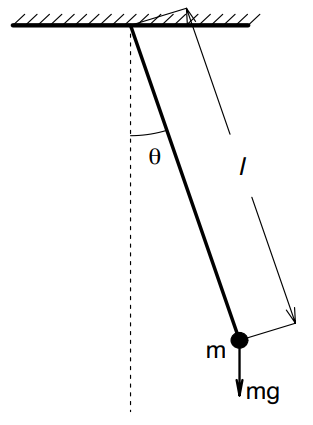
\includegraphics[height = 5cm]{Figures/Fig1.png}
				\caption{Simple pendulum of mass $m$ and length $l$ under the action of Earth’s gravitational force.}
			\end{figure}
		\end{enumerate}
	\end{problem}

	\begin{problem}{2}
		The SVD result of a matrix A is below
		\begin{verbatim}
		svdA=svd(A)
		
		svdA$d
		[1] 3.0 1.0
		
		svdA$u
     [,1] [,2]
		[1,]     0    1
		[2,]     1    0
		
		svdA$v
     [,1] [,2]
		[1,]   0.0    1
		[2,]   0.6    0
		[3,]   0.8    0

		\end{verbatim}
		\begin{enumerate}[label = (\alph*)]
			\item Write down three matrices $U, D, V$ in the $SVD$ formula $A = UDV'$ where $V'$ denotes the transpose matrix of $V$.
			\[\boldsymbol{U = \begin{bmatrix}
				0 & 1 \\ 1 & 0
			\end{bmatrix}, D = \begin{bmatrix}
				3.0 & 0 \\ 0 & 1.0
			\end{bmatrix}, V = \begin{bmatrix}
				0.0 & 1 \\ 0.6 & 0 \\ 0.8 & 0
			\end{bmatrix}}\]
			\item Use the $SVD$ formula $A = UDV'$ to recover the original matrix $A$ by hand calculation for the multiplication of the three matrices
			\begin{align*}
				\boldsymbol{A = UDV'} &= \boldsymbol{\begin{bmatrix}
						0 & 1 \\ 1 & 0
					\end{bmatrix}\begin{bmatrix}
						3.0 & 0 \\ 0 & 1.0
					\end{bmatrix}\begin{bmatrix}
						0.0 & 0.6 & 0.8 \\ 1 & 0 & 0 
					\end{bmatrix} = \begin{bmatrix}
						0 & 1.0 \\ 3.0 & 0 
					\end{bmatrix}\begin{bmatrix}
						0.0 & 0.6 & 0.8 \\ 1 & 0 & 0 
				\end{bmatrix}} \\
			&= \boldsymbol{\begin{bmatrix}
				1 & 0 & 0 \\ 0.0 & 1.8 & 2.4
			\end{bmatrix}}
			\end{align*}
		\end{enumerate}
	\end{problem}

	\begin{problem}{3}
		The Buffon’s needle problem: A needle of length $l$ is dropped onto a floor with equally spaced parallel lines, as shown in Figure 2. The distance between each nearby two lines is $d$.
		\begin{enumerate}[label = (\alph*)]
			\item  Derive the formula to calculate the probability of the needle crossing, or touching a line
			when $l < d$, i.e., the case of short needles. Express your formula in terms of $l$ and $d$.
			\\ \\
			\textit{Requirements: You must draw a diagram of a needle and two lines, clearly mark the needle’s position
			using symbols $y$ and $\theta$ for its relevant distance and angle. You must draw a figure on the $\theta - y$ plane
			to formulate a geometric probability problem. Write down the needle cross condition in terms of $y, \theta, d$
			and $l$.}
			\\ \\
			Notice the following:
			\\ \\
			Let $y$ be position of the lower end of the needle, $d$ be the gap between the two lines, and $\ell < d$ be the length of the needle.
			\\ \\
			We have the probability region be in the space $[-\pi/2, \pi/2] \times [0,d]$.  Thus we get the probability region is $A = \pi d$.
			\\ \\
			We can use the following equation to determine when the line will cross the top line:
			\[y + \ell \cos \theta \geq d, \qquad y \geq d - \ell \cos \theta  \]
			When $\theta = 0$, the line will cross the top line if $y \geq  d - \ell$.
			\\ 
			When $|\theta| = \pi /2$, the line will cross if $y = d$
			\\ \\
			Thus, we get that the area in which the line can be to cross the top line would be as long as $y < d$, and $y \geq d - \ell \cos \theta$
			\\ \\
			So we can calculate the probability of that happening with the following equation:
			\[P = \frac{1}{\pi\,d} \int_{-\pi/2}^{\pi/2} d - (d - \ell \cos \theta)\,d\theta = \frac{2\ell}{\pi\,d}\]
			\begin{figure}[h!]
				\centering
				\begin{subfigure}{.45\textwidth}
					\centering
					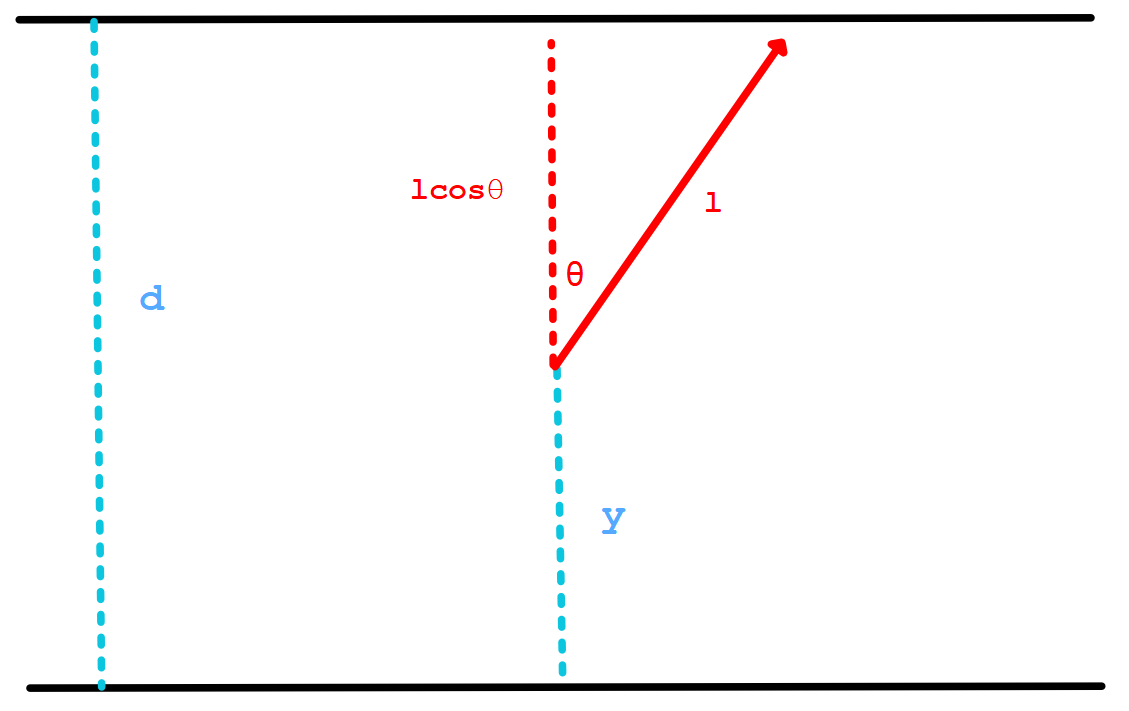
\includegraphics[height = 5cm]{Figures/needle}
				\end{subfigure}
				\begin{subfigure}{.45\textwidth}
					\centering
					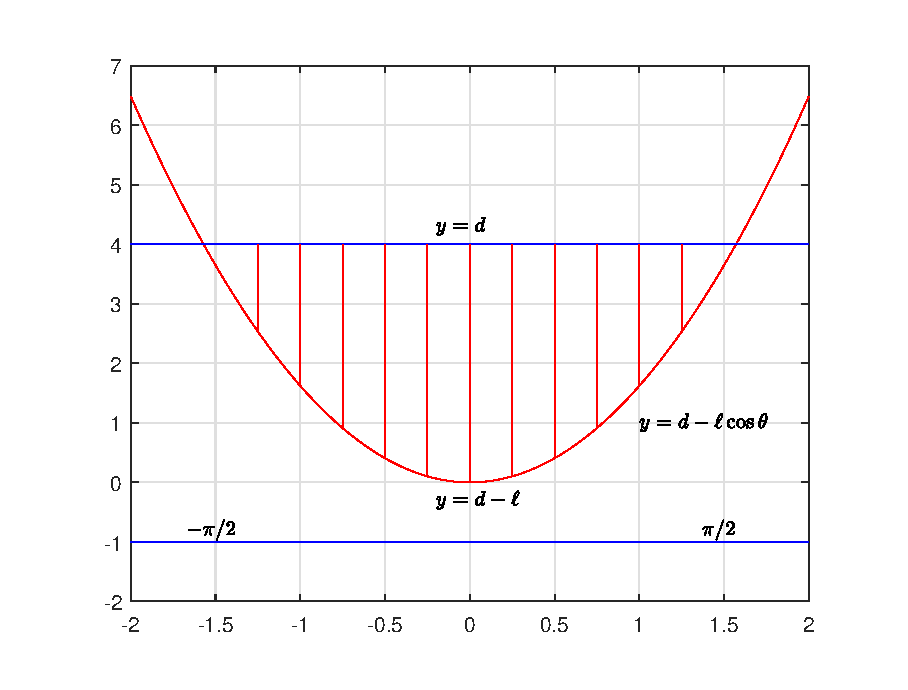
\includegraphics[height = 6cm]{Figures/Prob3a}
				\end{subfigure}
			\end{figure}
			\newpage
			\item  Compute the probability of crossing or touching when $l = 0.2$ $[meter]$ and $d =
			0.3$ $[meter]$.
			\[P = \frac{2\ell}{\pi\,d} = \frac{2(0.2)}{\pi\,(0.3)} = .4244 = 42.44\%\]
			\item  Given $d = 0.25$ $[meter]$, what is the needle length $l$ so that the the probability of crossing
			or touching is 0.5?
			\[P = \frac{2\ell}{\pi\,d} = \frac{2\ell}{\pi\,(0.25)} = 0.5, \qquad \ell = \frac{0.5\pi (0.25)}{2} = .1963\,\]
			\skipline
			\begin{figure}[h!]
				\centering
				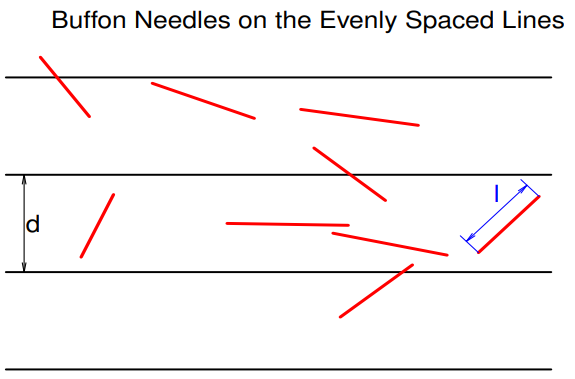
\includegraphics[height = 5cm]{Figures/Fig2.png}
				\caption{The Buffon’s needle problem: a geometric probability example.}
			\end{figure}
		\end{enumerate}
	\end{problem}

	\begin{problem}{4}
		\begin{enumerate}[label = (\alph*)]
			\item Derive a formula for the monthly mortgage payment $x$, expressed in terms of the principal
			amount $P$, monthly interest rate $r$, and total number of months of the loan $n$. Show your work and the
			detailed steps. The answer for this problem (a) is a formula.

			
			Let $P_k$ represent the principal amount owed after $k$ months, such that:
			\begin{align*}
				P_1 &= P(1 + r) - x \\
				P_2 &= P(1 + r)^2 - x(1 + r) - x \\
				P_3 &= P(1 + r)^3 - x(1 + r)^2 - x(1 + r) - x \\
				P_k &= P(1 + r)^k - x\sum_{i = 0}^{k-1} (1 + r) \\
				&= P(1 + r)^k  - x\left(\frac{1 - (1 + r)^k}{1 - (1 + r)}\right) \\
				&= P(1 + r)^k  + x\left(\frac{1 - (1 + r)^k}{r}\right) 
			\end{align*}
			Notice that at the end of $n$ months, the principal will be \$0, thus we get:
			\begin{align*}
				P_n = 0 &= P(1 + r)^n  + x\left(\frac{1 - (1 + r)^n}{r}\right) \\
				x\left(\frac{(1 + r)^n - 1}{r}\right) &= P(1 + r)^n \\
				\boldsymbol{x} &= \boldsymbol{\frac{P(1 + r)^nr}{(1 + r)^n - 1}}
			\end{align*}
			\newpage
			\item Given the following data: The principal amount (i.e., the total loan) is $P$ = \$400, 000, the
			annual interest rate is 3.0\% (converted into the monthly rate 0.25\%), and the loan is to be paid off in 30
			years (equivalent to 360 months). Use the above derived formula and the data to compute the monthly
			mortgage payment $x$ by a calculator or R. The answer should be an amount of money per month. You
			do not need to submit the R code for this problem.

			\[x = \frac{400,000(1 + .0025)^{360}(.0025)}{(1 + .0025)^{360} - 1} = \$1686.42\]
			\item If the annual rate is reduced to 2.95\% in the above data, what is the monthly mortgage payment?
			\\ \\
			With an annual rate of 2.95\%, the monthly rate becomes $r = .002458\%$.
			\[x = \frac{400,000(1 + .002458)^{360}(.002458)}{(1 + .002458)^{360} - 1} = \$1675.65\]
			\item  If the principal is increased to $P$ = \$470, 000, the annual rate is 2.875\%, and the loan
			period is still 30 years, what is the the monthly mortgage payment now?
			\\ \\
			With an annual rate of 2.875\%, the monthly rate becomes $r = .002396\%$.
			\[x = \frac{470,000(1 + .002396)^{360}(.002396)}{(1 + .002396)^{360} - 1} = \$1949.99\]
		\end{enumerate}
	\end{problem}

	\begin{problem}{5}
		\begin{enumerate}[label = (\roman*)]
			\item Use R to solve the following linear equations for $x_1, x_2, x_3, x_4$:
			\[\begin{cases}
				-x_1 + 2.9x_2 + x_3 - x_4 & = 1 \\
				-2.5x_1 -1.9x_2 + x_3  & =  2.1 \\
				2.1x_1 -3.8x_2 -4x_3 -3x_4 & = 0 \\
				x_1 - x_2 -3.1x_3 -8.6x_4 & = 2.5
			\end{cases}\]
			Copy your R solution result to your R code as comment lines after \#
\begin{lstlisting}[language=R]
a = c(-1,-2.5,2.1,1, 2.9,-1.9,-3.8,-1,  1,1,-4,-3.1, -1,0,-3,-8.6)
b = c(1, 2.1, 0, 2.5)

A = matrix(a , ncol=4)
B = matrix(b,ncol = 1)

C = solve(A,b)
# x1            x2          x3           x4
# -0.963747260  0.009707986 -0.290922978 -0.299022560
\end{lstlisting}
			\skipline
			\item Write an R code of Monte Carlo simulation to approximately evaluate the volume of a ball of radius
			equal to 1.0 in 6-dimensional space. Please use at least 100,000 points.
\begin{lstlisting}[language=R]
MCSim = function(dim, n = 1e6) {
	x = matrix(runif(dim*n, min= -1, max = 1), ncol = dim)
	k = 0
	for (i in 1 : n) {
		if ( (t(x[i,]) %*% x[i,]) < 1) { k = k + 1 }
	}
	return( (k/n) * 2^dim )
}

MCExact = function(n,R=1) {
	numer = pi^(n/2)
	denom = gamma((n/2) + 1)
	return((numer/denom)*(R^n))
}


MCSim(6, 1e6) # 5.16736
MCExact(6)    # 5.167713
\end{lstlisting}
			\newpage
			\item Use Monte Carlo method to approximately evaluate the following integral
			\[\int_1^2 \frac{1 - x^2 + 9\cos x}{x(1 + x + \sin x)}\,dx \tag{(0.1)}\]
			Please use at least 100,000 points.
\begin{lstlisting}[language=R]
integrateMc = function(f, lowBound, highBound, n = 1e6) {
	x = runif(n , lowBound, highBound)
	return ((highBound - lowBound) * mean(f(x)))
}


f = function(x) { (1 - (x^2) + (9*cos(x)) ) / ( x*( 1 + x + sin(x) ) )}

integrateMc(f, 1, 2, 1e6)   # 0.05252009
integrate(f,1,2)            # 0.05297656
\end{lstlisting}
			\item Figure 3 shows the history of the global average December mean temperature anomalies. Use R and the dataset \codefont{EarthTemperatureData.txt} or \codefont{EarthTemperatureData.csv}
			downloadable from BB’s Assignment/Final Exam block to plot a similar figure but for November and
			with the following requirements.
			\begin{enumerate}[label = (\alph*)]
				\item Replace "Samuel Shen" and "December" in the main title by your name and November.
				\item Change the curve’s color from black to orange and use \codefont{lwd=3}.
				\item  Compute the linear trend of the November temperature anomalies for the period from 1901 to 2000
				using R command \codefont{lm( )}. Please note that this is NOT the entire data time period of 1850-2015.
				Hint: See Fig. 3.6 in the textbook for reference.
				\item Plot the trend line from 1901 to 2000 in the blue color. The blue trend line must be limited within
				the time period of 1901-2000, not the entire data time period of 1850-2015. Use \codefont{lwd=3}. for the trend
				line.

				\item Change the text "December trend = 0.52 deg C/century" to "1901-2000 November trend = ?? deg C
				per century", and use the trend calculated from Step (c) in the position "??".
				\item[(g)] Find the hottest and coldest November temperature anomalies. Which years did they occur?
				\\ \\
				We got the coolest November temperature anomaly of $-0.753^\circ C$ in the year 1862. 
				\\ \\
				We got the hottest November temperature anomaly of $0.81^\circ C$ in the year 2015. 
				\newpage
\begin{lstlisting}[language=R]
time = matrix(readData['YEAR'][[1]],nrow = 1)
NovData = matrix(readData['NOV'][[1]],nrow = 1)

plot(time, NovData, 'l',main = 'Stephen Giangs plot of November Temperature Anomalies',  ylab = 'Temperature [deg C]', 
    xlab = 'Year', col = 'orange', lwd = 3)

trendLineData = subset(readData, YEAR >= 1901 & YEAR <= 2000)
tlTime = trendLineData['YEAR'][[1]]
tlNov = trendLineData['NOV'][[1]]
linMod = lm(tlNov ~ tlTime)
intercept = linMod$coefficients[1]
slope = linMod$coefficients[2]

tL = slope*tlTime + intercept
lines(tlTime, tL, col = 'blue', lwd = 3)

trendLabel = paste0('1901 - 2000 November Trend = ', round(slope * 100,4), ' deg C per Century')
text(1900, .5, trendLabel)

minTemp = min(NovData)                      # -0.753
minTime = 1849 + which(NovData == minTemp)  # 1862
maxTemp = max(NovData)                      # 0.81
maxTime = 1849 + which(NovData == maxTemp)  # 2015
\end{lstlisting}
				\begin{figure}[h!]
					\centering
					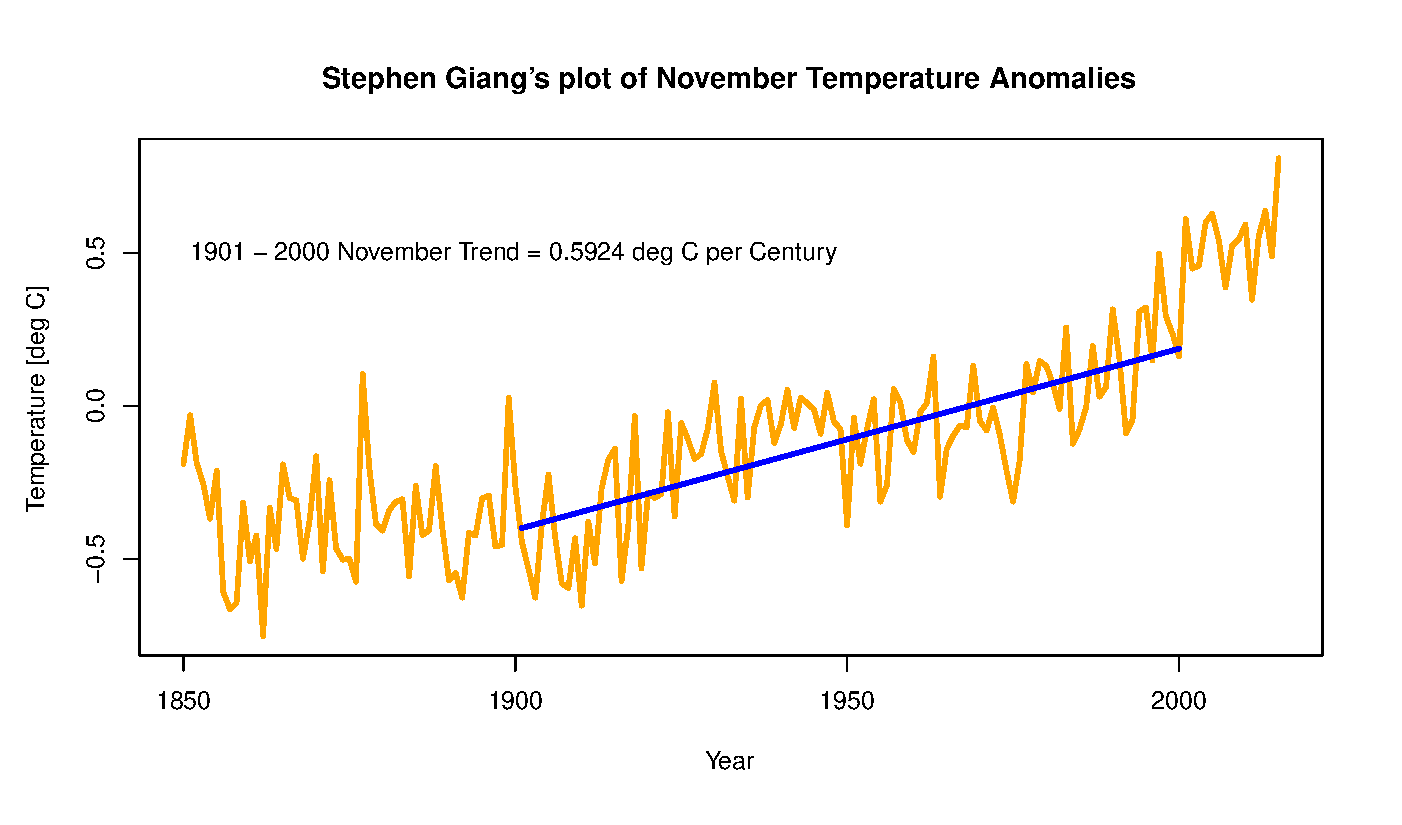
\includegraphics[width = \textwidth]{Figures/Prob54}
				\end{figure}
				\newpage
				\begin{figure}[h!]
					\centering
					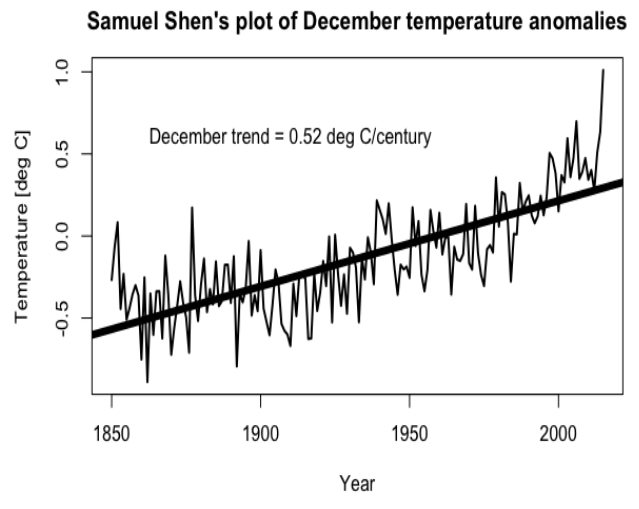
\includegraphics[height = 8cm]{Figures/Fig3.png}
					\caption{Global average December mean global average surface air temperature anomalies from 1850-2015.}
				\end{figure}
			\end{enumerate}
			
		\end{enumerate}
	\end{problem}

\end{document}
